\section{Роль усилителя мощности и влияние нелинейности
на характеристики различных сигналов}
Усилитель мощности (УМ) является ключевым компонентом передатчика,
отвечающим за повышение мощности сигнала, передаваемого устройством или
базовой станцией. УМ также является одним из элементов цепи передатчика с
самым высоким энергопотреблением. Чем больше необходимо усилить сигнал, тем
больше энергии необходимо УМ. Однако при этом, при высокой мощности,
поведение УМ становится нелинейным. Известно, что эффективность УМ,
работающего в радиочастотном диапазоне (RF), может значительно повлиять на
производительность всей передающей системы
в целом \cite{Lie2018}.

В этой главе рассматривается основной принцип работы УМ, влияние
нелинейности на усиливаемый сигнал и математические модели основных
характеристик.


\subsection{Описание принципа работы усилителя мощности}
Одной из основных характеристик УМ является коэффициент усиления (КУ) $G$,
который определяется как отношение выходной мощности $P_{out}$ к входной
$P_{in}$. Часто выражается в дБ:
\begin{equation}
    G_{dB} = 10\log_{10}\left(\frac{P_{out}}{P_{in}}\right)
\end{equation}
КУ УМ зависит от множества факторов, в том числе от свойств элементов,
использованных для создания УМ. Реальный УМ - это нелинейное устройство, КУ
которого не постоянен. Напротив, КУ сильно зависит от свойств
индивидуальных составляющих, входной мощности, частоты сигнала и других
параметров. Однако часто считают, что в некотором диапазоне входных
мощностей и частот КУ является постоянным или достаточно слабо
меняющимся.

Помимо КУ, усилитель мощности часто описывается при помощи двух функций —
амплитудная характеристика (АХ) $F_{AM/AM}$ и фазовая характеристика (ФХ)
$F_{AM/PM}$. Амплитудная характеристика определяет зависимость значения
амплитуды сигнала (напряжения, тока или мощности) на выходе $U_{out}$ от
значения амплитуды сигнала на входе $U_{in}$. Фазовая характеристика
определяет величину сдвига фазы $\Delta\phi$ выходного сигнала относительно
входного в зависимости от амплитуды сигнала на входе $U_{in}$.
\begin{equation}
    U_{out} = F_{AM/AM}(U_{in}), \quad \Delta\phi = F_{AM/PM}(U_{in})
\end{equation}

Для удобства описания и анализа сигнала часто прибегают к использованию
нотации комплексной огибающей $\tilde{x}(t)$. Тогда входной сигнал может быть
записан как 
\begin{equation}
    x(t) = \tilde{x}(t) \cdot \exp(i \omega_c t),
\end{equation}
где $\omega_c$ - частота несущей, $i$ - мнимая единица, $t$ - время.
Комплексная огибающая $\tilde{x}(t)$ имеет следующий вид:
\begin{equation}
    \tilde{x}(t) = a(t) \exp(i\phi(t)),
\end{equation}
где $a(t)$ - амплитуда, $\phi(t)$ - фаза входного сигнала. Отклик УМ $y(t)$
в таком случае будет усиленной и искаженной версией $x(t)$, который может
быть записан как
\begin{equation}
    \begin{aligned}
        &y(t) = \tilde{y}(t) \cdot \exp(i \omega_c t)\\
        &\tilde{y}(t) = F_{AM/AM}(a(t)) \cdot \exp[i \phi(t) + F_{AM/PM}(a(t))].
    \end{aligned}
    \label{eq:pa_distortion}
\end{equation}

В случае идеального УМ, амплитудная характеристика имеет вид прямой (см.
Рис.\ref{fig:1.1}a), пересекающейся с началом координат. Это означает, что
коэффициент усиления линейного (идеального) усилителя постоянен и не
зависит от входного сигнала. Коэффициент усиления идеального УМ может быть
определен как тангенс угла наклона АХ к оси абсцисс.

\begin{figure}[h!]
    \centering
    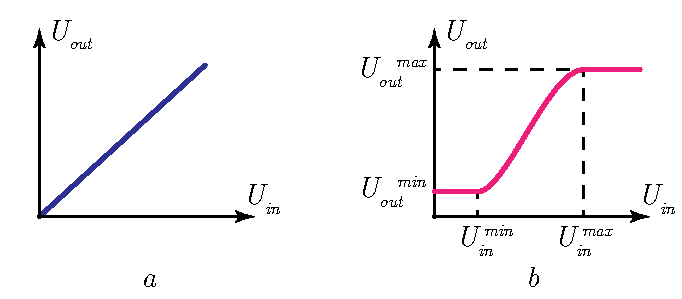
\includegraphics[width=0.8\linewidth]{figs/amp_char.pdf}
    \caption{Амплитудные характеристики идеального и реального усилителя мощности}
    \label{fig:1.1}
\end{figure}

Однако как наблюдается на практике, АХ усилителей редко бывают линейными,
ввиду множества факторов, обуславливающих нелинейность этой характеристики
(см. Рис. \ref{fig:1.1}б). При нулевом напряжении на входе, на выходе
усилителя присутствует ненулевое напряжение, обусловленное собственными
шумами усилителя. Из-за этого появляется изгиб в нижней части АХ. При
достаточно больших значениях входной амплитуды, АХ также отклоняется от
прямой. Из-за выхода рабочей точки отдельных элементов усилителя за пределы
рабочего диапазона, возникают нелинейные искажения, вследствие которых
коэффициент усиления сигнала выходит на уровень насыщения.

При этом, АХ реального УМ имеет определенный диапазон входных значений
амплитуд $(U_{in}^{min},U_{in}^{max},)$, при которых искажения практически
отсутствуют и усилитель подобен идеальному. Эта область называется
\textit{динамическим диапазоном усилителя} и выражается как
\begin{equation}
    D = \frac{U_{in}^{max}}{U_{in}^{min}}.
\end{equation}

В связи с ограниченностью динамического диапазона УМ, часто изменяют
входной сигнал таким образом, чтобы итоговая рабочая точка находилась в
нужном диапазоне линейности и усиления. Используется смещение рабочей точки
относительно выходной мощности - OBO (\textit{Англ. - Output back-off}), и
смещение рабочей точки относительно входной мощности - IBO (\textit{Англ. -
Input back-off})(см. рис. \ref{fig:obo_ibo}). При этом обычно
представляется возможным пересчет одной величины в другую, так как по сути
они являются взаимозаменяемыми. Разница состоит в том, относительно чего
происходит сдвиг рабочей точки - максимальной выходной, либо максимальной
входной мощности.

\begin{figure}[h!]
    \centering
    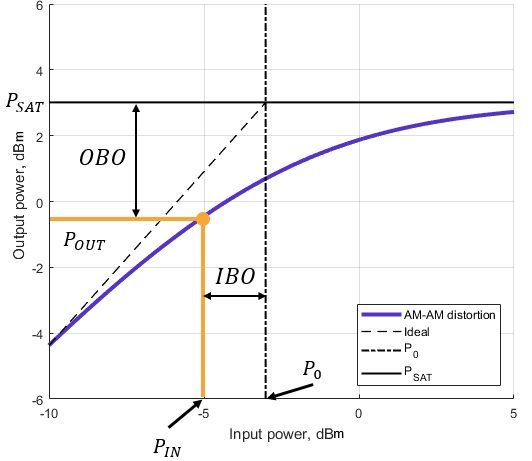
\includegraphics[width=0.7\linewidth]{figs/pa_obo_ibo.png}
    \caption{Смещение рабочей точки усилителя относительно входной (IBO) и выходной мощности (OBO).}
    \label{fig:obo_ibo}
\end{figure}

\begin{equation}
    OBO = 10 \cdot \log_{10}\left(\frac{P_{sat}}{P_{out}}\right), \quad
    IBO = 10 \cdot \log_{10}\left(\frac{P_{0}}{P_{in}}\right)
\end{equation}

Большие значения IBO\slash OBO могут обеспечить хорошую линейность АХ,
однако это также приведет к уменьшению средней выходной мощности сигнала.
Таким образом, в реальных применениях определяется наиболее подходящее
значение IBO \slash OBO, обеспечивающее необходимую линейность
характеристики, а также необходимое усиление.


\subsection{Нелинейность и искажение сигналов}
Мощность на выходе УМ увеличивается вместе с ростом входной мощности,
однако, как только уровень выходной мощность достигает определенного
максимума, КУ перестает быть постоянным и усилитель входит в область
насыщения. В этой области больше всего проявляется нелинейность УМ -
выходная мощность перестает увеличиваться с ростом входной мощности. Работа
УМ в нелинейной области влечет за собой нелинейные искажения сигнала,
которые заключаются в изменение его формы и фазы.

В качестве входного рассмотрим сигнал с гармонически меняющейся амплитудной
(мощностью $P_{in}$) (см. рис \ref{fig:pa_distortion_sin}). Если УМ
находится в линейном режиме работы, то на выходе также будет гармонический
сигнал, отличающаяся только усилением амплитуды. Однако если усилитель
находится в нелинейной области, на выходе сигнал будет отличаться от
входного не только значением амплитуды, но и формой. Пики синусоиды будут
сжиматься нелинейной частью АХ, что приведет к искажению сигнала на выходе
(см. рис \ref{fig:pa_distortion_sin}).

\begin{figure}[h!]
    \centering
    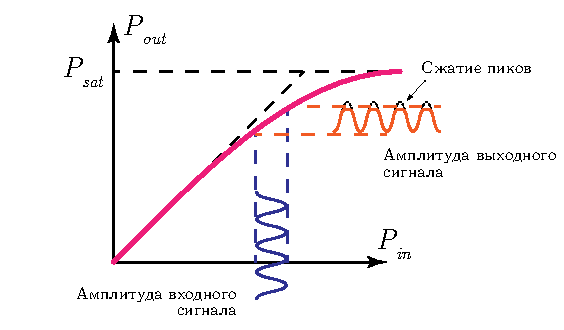
\includegraphics[scale=1.2]{figs/amp_dist.pdf}
    \caption{Преобразование сигнала с гармонически меняющейся амплитудой при прохождении через УМ}
    \label{fig:pa_distortion_sin}
\end{figure}

% А вот хер знает, тут не уверен

% Сжатие пиков во временной области будет также приводить к искажениям и
% изменениям в частотной области, а именно к росту ширины спектра. Изначально
% подаваемый сигнал имеет очень узкий спектр (дельта-функция на несущей
% частоте) 

% \begin{figure}[h!]
%     \centering
%     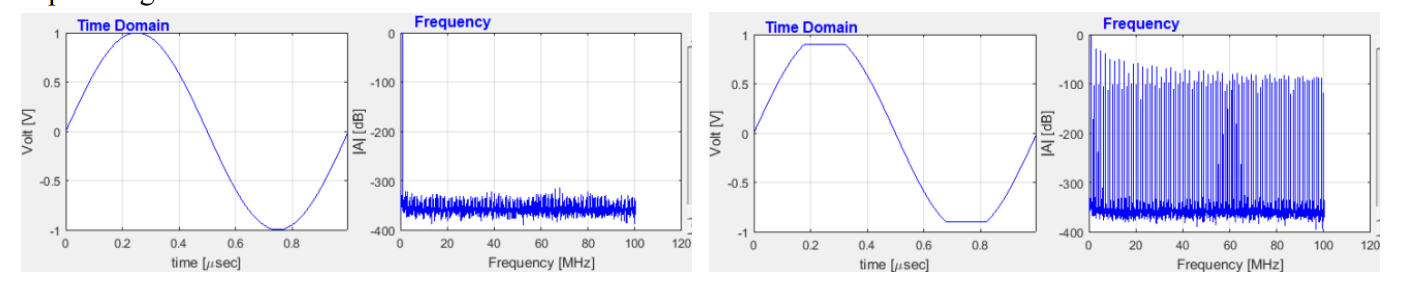
\includegraphics[width=0.9\linewidth]{figs/pa_spectral_growth.png}
%     \caption{Влияние сжатия пиков на частотную область сигнала}
%     \label{fig:pa_distortion_freq}
% \end{figure}

Рассмотрим влияние нелинейности характеристики усилителя на основные типы
сигналов, часть которых используется в стандарте 5G NR.

\begin{figure}[h!]
    \centering
    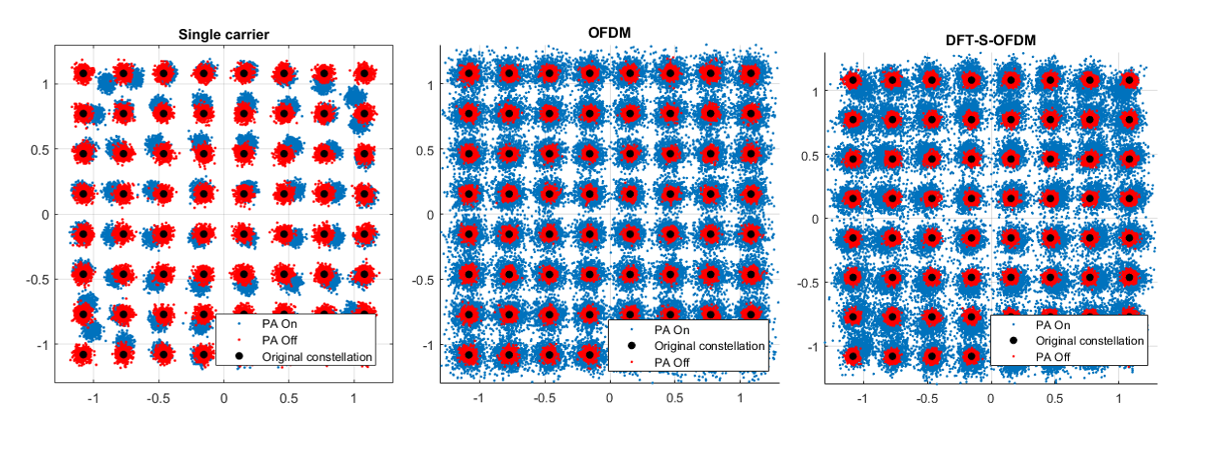
\includegraphics[width=0.98\linewidth]{figs/ofdm_pa_distortions.png}
    \caption{Искажение различных сигналов на приемнике при внесении нелинейного
    искажения на передатчике}
    \label{fig:lls_rapp_distortions_0}
\end{figure}

Для примера рабочая точка (средняя входная мощность) была выбрана так,
чтобы влияние нелинейности амплитудной характеристики усилителя была
достаточно явна продемонстрирована.
\subsubsection{Single Carrier}
\begin{figure}[h!]
    \centering
    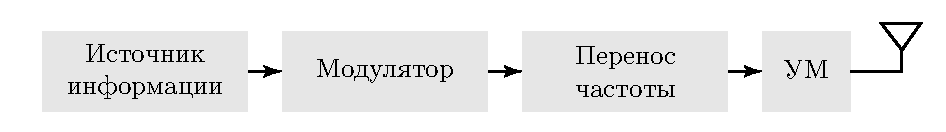
\includegraphics[scale=1]{figs/sc_scheme.pdf}
    \caption{Принципиальная схема генерации SC-сигнала}
    \label{fig:sc_scheme}
\end{figure}
\textit{Single Carrier} - SC сигнал с одной несущей, передаваемые данные
кодируются с помощью модуляции (BPSK, QPSK, N-QAM) в виде амплитуды сигнала
на несущей частоте. Схема генерации SC-сигнала приведена на рис.
\ref{fig:sc_scheme}. Отметим, что SC сигналом часто называют SC-FDMA
сигнал, который в стандарте 5G-NR получил название DFT-s-OFDM.

Поскольку на усилитель подается, по сути, амплитудно модулированный сигнал,
то искажения имеют достаточно предсказуемый характер. На рис.
\ref{fig:lls_rapp_distortions_0}a приведен график созвездия модуляции
64-QAM, который в данном случае используется для сигнала SC. Черные точки
показывают изначальное местоположение созвездия, красные - созвездия на
приемнике с использованием идеального усилителя мощности, синие - созвездия
на приемнике с использованием нелинейного усилителя мощности. 

Наблюдаемая картина напоминает искажение амплитуды на рис.
\ref{fig:pa_distortion_sin}, т.е. искажение обработанного сигнала напрямую
связано с его амплитудой - чем больше амплитуда, тем больше искажение.
Такой тип сигнала имеет детерминированный характер искажения нелинейностью,
и может, в теории, быть достаточно просто компенсирован.


\subsubsection{OFDM / CP-OFDM}
\textit{Orthogonal Frequency-Division Multiplexing} - OFDM сигнал,
использующий большое число близко расположенных ортогональных поднесущих,
каждая из которых модулируется по стандартной схему модуляции (аналогично
SC). В стандарте 5G NR часто используется \textit{CP}-OFDM - \textit{Cyclic
Prefix} OFDM - сигнал OFDM с добавлением цикличного префикса. CP необходим
для борьбы с межсимвольной интерференцией (ISI), и заключается в создании
меж-символьного защитного интервала, состоящего из копии части
OFDM-символа. Принципиальная схема генерации OFDM сигнала приведена на рис.
\ref{fig:ofdm_scheme}. OFDM сигнал принципиально отличается от SC сигнала,
поток данных делится на несколько параллельных подпотоков с более низкой
скоростью передачи (увеличение длительности символа), а каждый поток
модулируется на своей ортогональной поднесущей. OFDM также достаточно прост
в обработке, чаще всего применяется прямое и обратное преобразование Фурье,
с помощью которого происходит перенос сигнала между частотной и временной
областью.
\begin{figure}[h!]
    \centering
    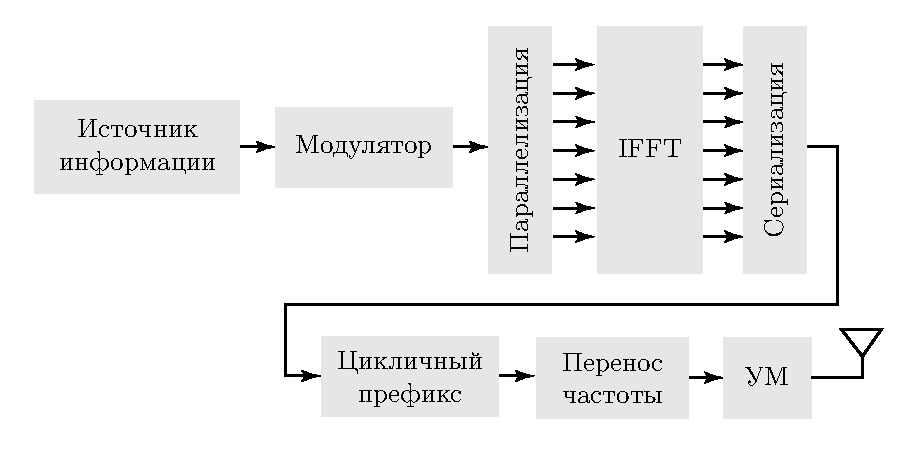
\includegraphics[scale=1]{figs/ofdm_scheme.pdf}
    \caption{Принципиальная схема генерации CP-OFDM-сигнала.
    \textbf{M}-IFFT означает что операция IFFT производится по M точкам.}
    \label{fig:ofdm_scheme}
\end{figure}

Что касается искажения при прохождении через нелинейный УМ, ввиду наличия
операции IFFT (на передатчике) перед усилителем, результирующие искажения
на приемнике после преобразования OFDM-сигнала в созвездие с помощью FFT
имеют достаточно сложный и непредсказуемый характер, как и это предложение.
Пример искажений OFDM-сигнала изображен на рис.
\ref{fig:lls_rapp_distortions_0}b. Из графика видно, что размер облака
точек вокруг точек созвездий увеличивается при присутствии нелинейного
усилителя в цепи передатчика (синие точки), однако отсутствует
централизованный сдвиг облаков относительно изначальных положений. 

Таким образом, искажения CP-OFDM сигнала носят недетерминированный
характер, в какой-то степени случайный. Такие искажения может быть
проблематично компенсировать.

\subsubsection{DFT-s-OFDM}
\textit{(Discrete) Fourier Transform Spread OFDM} - DFT-s-OFDM сигнал
является модификацией сигнала OFDM, нацеленной на компенсацию его основного
недостатка, а именно высокого отношения пикового уровня мощности к среднему
(\textit{Англ. - Peak to Average Power Ratio - PAPR}). Подробнее проблема
высокого PAPR рассмотрена в секции \ref{sec:papr}. Принципиальная схема
генерации DFT-s-OFDM сигнала приведена на рис. \ref{fig:dfts_scheme}.
\begin{figure}[h!]
    \centering
    % 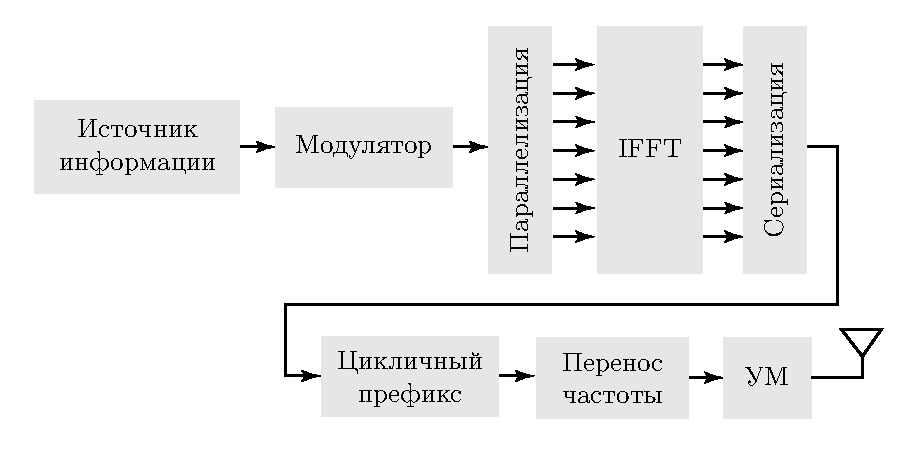
\includegraphics[scale=1]{figs/ofdm_scheme.pdf}
    % \includegraphics[scale=0.8]{example-image-a}
    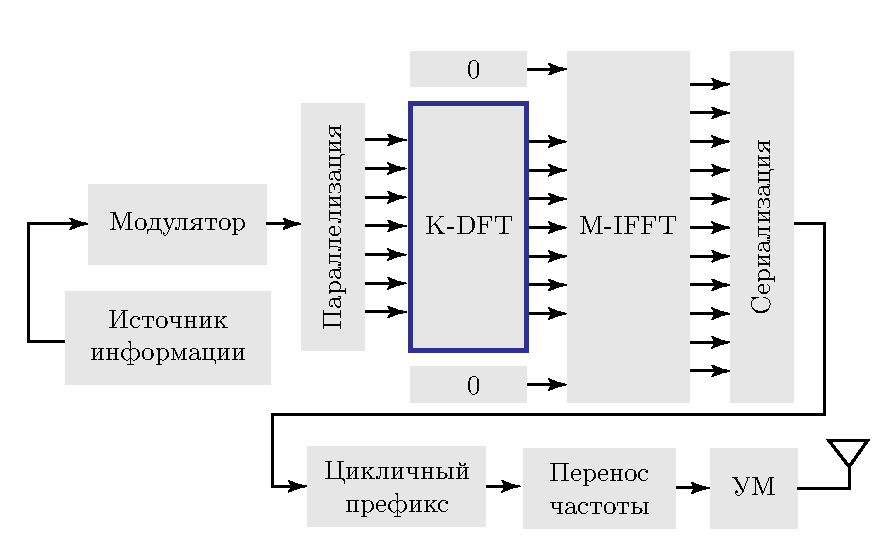
\includegraphics[scale=1]{figs/dfts_scheme.pdf}
    \caption{Принципиальная схема генерации DFT-s-OFDM-сигнала.
    \textbf{K}-DFT означает что операция DFT производится по K точкам.}
    \label{fig:dfts_scheme}
\end{figure}
Генерация DFT-s-OFDM сигнала отличается от классического OFDM включением
предварительного кодирования параллелизованного потока данных при помощи
прямого дискретного преобразования Фурье (DFT, FFT), примененного к
ограниченному количеству поднесущих OFDM сигнала ($K<M$). В стандарте 3GPP
данная операция называется \textit{Transform Precoding}. По своей сути
эта процедура повторяет принцип, применяемый в SC-FDMA. За счет
сочетания Transform Precoding и IFFT, присутствующего в процедуре создания
OFDM сигнала, полученный сигнал имеет меньшие значения PAPR, тем самым
более эффективно используя ограниченный диапазон работы усилителя.

Поскольку DFT-s-OFDM сигнал является неким средним между CP-OFDM и SC,
искажения, вносимые нелинейностью УМ имеют также смешанный характер. Пример
таких искажений приведен на рис. \ref{fig:lls_rapp_distortions_0}c.
Присутствует как общее смещение облаков созвездия ввиду амплитудных
искажений, так и увеличение разброса по сравнению со случаем
использования идеального (линейного) усилителя.

\subsection{Проблема пик-фактора PAPR сигнала OFDM}
\label{sec:papr}
Одним из недостатков сигнала OFDM является высокое отношение пиковой
мощности к средней - PAPR (пик-фактор). Визуализация этого отношения приведена на рис.
\ref{fig:papr}. В случае OFDM сигнала, высокое значение PAPR получается в
результате комбинации большого количества поднесущих, которые могут
когерентно сложиться, что и даст высокое значение пиковой мощности.
 
\begin{figure}[h!]
    \centering
    % 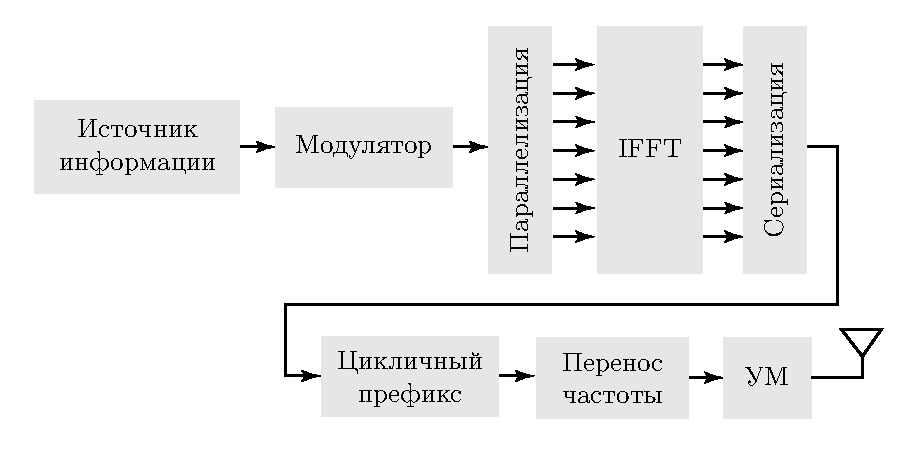
\includegraphics[scale=1]{figs/ofdm_scheme.pdf}
    % 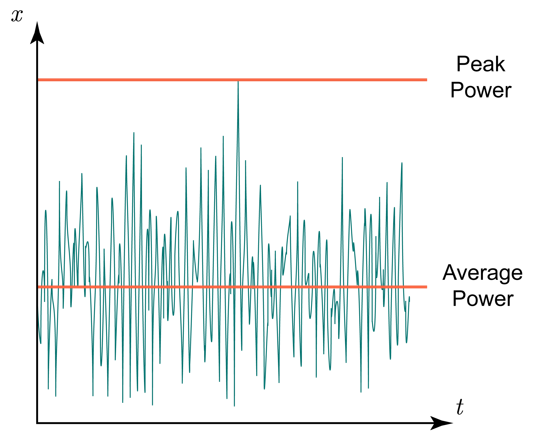
\includegraphics[width=0.49\linewidth]{figs/papr_scheme.png}
    % 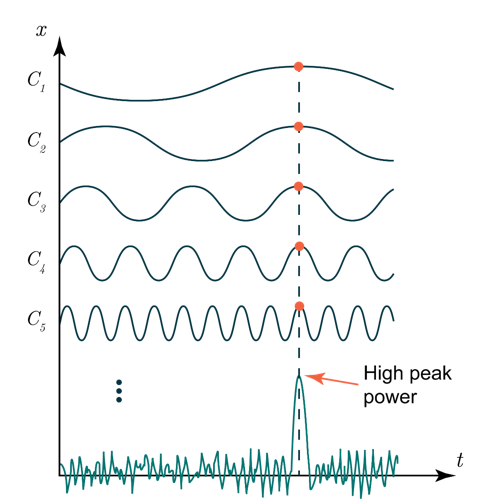
\includegraphics[width=0.49\linewidth]{figs/papr_ofdm.png}
    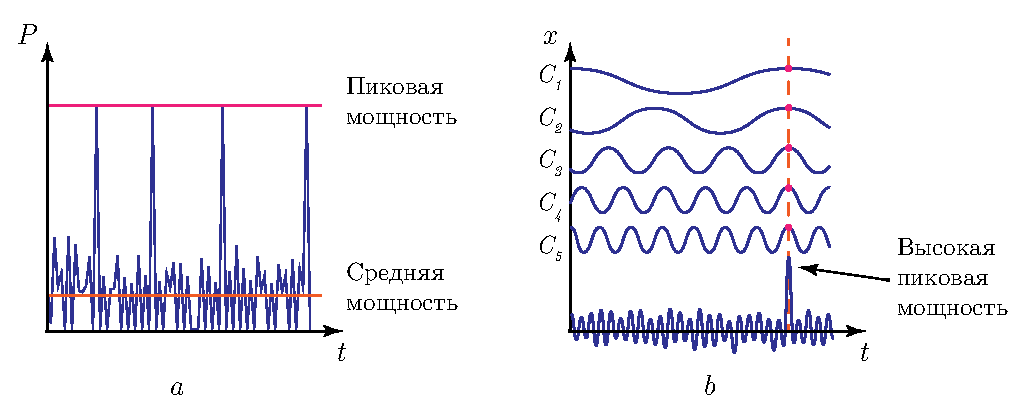
\includegraphics[scale=1]{figs/papr_explanation.pdf}
    \caption{Демонстрация отношения пиковой мощности к сигнала к средней
    мощности (слева) и принцип появления высокого PAPR у OFDM
    сигнала (справа). При комбинации большого количества гармоник возможно
    их сложение в фазе, что приведет к скачку мощности.}
    \label{fig:papr}
\end{figure}
Высокое значение PAPR негативно влияет на работу системы в целом, поскольку
напрямую влияет на выбор рабочей точки усилителя. Перед подачей на УМ,
сигнал должен быть настроен таким образом, чтобы его средняя мощность,
определяющая рабочую точку, соответствовала желаемому режиму работы
усилителя. Если отношение PAPR высокое, то при выбранной на основе средней
мощности рабочей точки, части сигнала с пиковой мощностью будут попадать на
сильно нелинейную часть характеристики усилителя, что приведет к
искажению. Для избежания негативных эффектов, часто сдвигают рабочую точку
таким образом, чтобы сигнал не искажался, однако вместе с этим также
понижается общая выходная мощность.

В стандарте LTE при передаче данных от пользователя к базовой станции
(\textit{Uplink}) используется сигнал SC-FDMA \cite{3gpp.36.211}, поскольку
высокое значение пик-фактора на мобильных устройствах не приемлемо. В
стандарте 5G NR, в качестве альтернативы OFDM в uplink используется сигнал
DFT-s-OFDM \cite{3gpp.38.300}. Эти сигналы отличаются пониженным значением
пик фактора \cite{Vaigandla2021}, что позволяет более эффективно
использовать УМ.


\subsection{Математическое описание характеристик реальных УМ}

Для моделирования использования УМ в системах мобильной связи часто прибегают к
математическим моделям, описывающим поведение сигнала (усиление, искажение) при 
прохождении через УМ. Исторически модели разделяются на две основных
группы - \textbf{физические} и \textbf{эмпирические} модели \cite{cambridge2008}.

Физические модели требуют знания внутренних электронных компонентов УМ, их
связи, а так же теории, описывающей их взаимодействие. Такие модели подходят
для симуляций на уровне схемы благодаря высокой точности, однако требуют
много вычислительных мощностей и времени, а также детальное описание
структуры и компонентов УМ.

Эмпирические модели используются, когда не известна внутренняя структура УМ,
или когда рассматривается системный уровень моделирования. Эти модели
основаны на результатах измерений и исследований конкретных УМ, на основе
которых были выведены зависимости снятых характеристик УМ (АХ, ФХ) от его
параметров.

Поскольку в данной работе исследуется возможность компенсации нелинейного
искажения на приемнике, то использоваться будет эмпирическая
(поведенческая) модель УМ. Среди таких моделей можно назвать
\textit{Volterra, Saleh, Ghorbani}, а также модели, представляющие собой комбинации
полиномиальных моделей. Все они являются достаточно простыми моделями,
которые отражают нелинейную природу УМ. Простота позволяет оперировать
меньшим количеством параметров усилителя, упрощая обработку в целом. Однако
такие модели не могут быть использованы для описания сложных усилителей,
таки как усилитель \textit{Doherty} \cite{Doherty1936}\cite{3gpp.38.803}.

С другой стороны, в рамках рассматриваемой задачи, а именно компенсации
искажений, внесенных на передатчике из-за нелинейности УМ, использование
более простой модели может быть оправдано. Целью данной работы является
создание метода компенсации нелинейных искажений на приемнике, с основным
мотивом минимизировать обработку на передатчике, а также стоимость
конечного устройства. Рассматриваются именно простые, мало размерные,
дешевые в производстве передатчики, в которых усилитель часто имеет далеко
не лучшие параметры и не отличается высокой эффективностью.

\subsubsection{Модель Раппа}
\begin{figure}[h!]
    \centering
    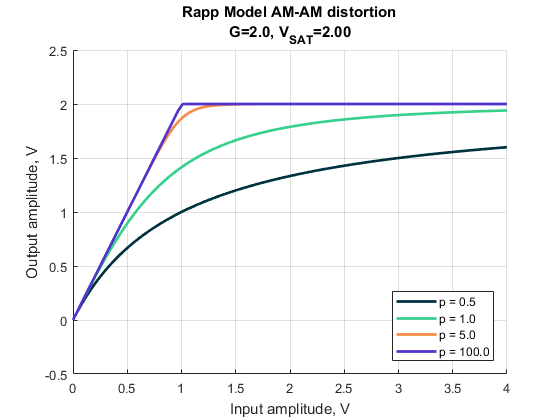
\includegraphics[width=0.7\linewidth]{figs/rapp_p.png}
    \caption{Влияние параметра гладкости $p$ на вид амплитудной
    характеристики (Добавить вторую и третью картинку где будут менять G, V)}
    \label{fig:rapp_p_parameters}
\end{figure}
Для описания искажения амплитуды и фазы при использовании твердотельных УМ
широко используется модель Раппа (\textit{Англ. - Rapp}) \cite{Rapp1991} \cite{Maltsev2010}.
Также существует модифицированная модель Раппа, приведенная в выражении
\ref{eq:Rapp}. Данная модель УМ включена в список моделей в спецификации
3GPP \cite{3gpp.38.803}.

\begin{equation}
    F_{AM/AM}(x) = \frac{G x}{\left( 1 + \abs{\frac{Gx}{V_{sat}}}^{2p}\right)^{1/2p}},
    \quad 
    F_{AM/PM}(x) = \frac{Ax^q}{\left(1+\left(\frac{x}{B}\right)^q\right)},
    \label{eq:Rapp}
\end{equation}
где $F_{AM/AM}, F_{AM/PM}$ - амплитудные и фазовые характеристики
соответственно, $G$ - КУ слабого сигнала, $V_{sat}$ - амплитуда насыщения,
$p$ - показатель гладкости характеристики. Параметры $A,B,q$ - параметры
кривой искажения фазы. В дальнейшем в работе будет использоваться эта
модель для описания влияния УМ на сигнал.

Пример АХ и ФХ для модели Раппа приведены на  рис. \ref{fig:rapp_p_parameters}.
В зависимости от значений параметров $G, V_{sat}, p$ поведение амплитудной
характеристики может сильно варьироваться. Так, при больших значениях $p$
($p\gg 1$), АХ похожа на характеристику идеального УМ, которая ограничена
по максимальной выходной амплитуде (см. рис. \ref{fig:rapp_p_parameters}).
Параметр $V_{sat}$ отвечает за выходную амплитуду насыщения, а $G$ - КУ
слабого сигнала.


\subsubsection{Параметры модели Раппа для диапазона 30-70 ГГц}
Для вывода параметров базовой модели УМ в диапазоне частот 30-70 ГГц,
компанией Nokia были использованы и исследованы характеристики стандартных
усилителей в соответствующей полосе \cite{nokia163314} \cite{Maltsev2010}.
Полученная модель УМ использована в этой работе для моделирования влияния
нелинейности УМ для сигналов с несущей частотой в диапазоне 30-70 ГГц.
Амплитудные и частотные характеристики УМ в соответствии с моделью
\cite{nokia163314} для 30-70 ГГц приведены на рис. \ref{fig:rapp_nokia}.
Численные значения параметров модели Раппа приведены в \ref{eq:rapp_p3070}.

\begin{equation}
    G = 16, \quad V_{sat} = 1.9, \quad p = 1.1
    \label{eq:rapp_p3070}
\end{equation}

\begin{figure}[h!]
    \centering
    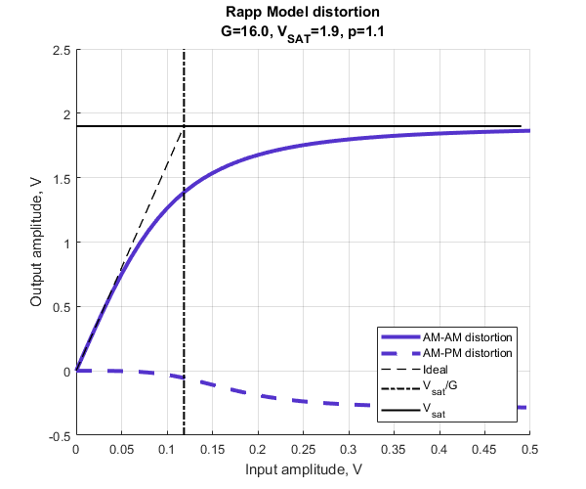
\includegraphics[width=0.7\linewidth]{figs/rapp_nokia.png}
    \caption{АХ и ФХ усилителя в соответствии с моделью Раппа и
    параметрами для диапазона 30-70 ГГц}
    \label{fig:rapp_nokia}
\end{figure}

\subsection{Характеристики УМ в миллиметровом диапазоне}
Помимо исследования диапазона частот 30-70 ГГц, в рамках данной работы
рассматривалось влияние нелинейного усилителя на качество приема для
диапазона миллиметровых длин волн, а именно 100-200 ГГц. Поскольку на
момент проведения исследования модель УМ для данного диапазона
отсутствовала, были изучены многочисленные отчеты и исследования с
указанием амплитудных характеристик используемых усилителей. Основываясь на
работах \cite{zhang2021}\cite{amadorey2018}\cite{aliyun2020} был сделан
вывод о значительном отличии характеристик УМ в более высоком диапазоне
частот. В целом, рассматриваемые усилители имею значительно меньшее
значение амплитуды насыщения $V_{sat}$ (или мощности насыщения), а также
меньшее значение коэффициента усиления $G$.

Характеристики твердотельных УМ из работ
\cite{zhang2021}\cite{amadorey2018}\cite{aliyun2020} приведены на рис.
\ref{fig:pa_research_mean}. Также на рис. \ref{fig:pa_research_mean}
приведена модель для 30-70 ГГц.
\begin{figure}[h]
    \centering
    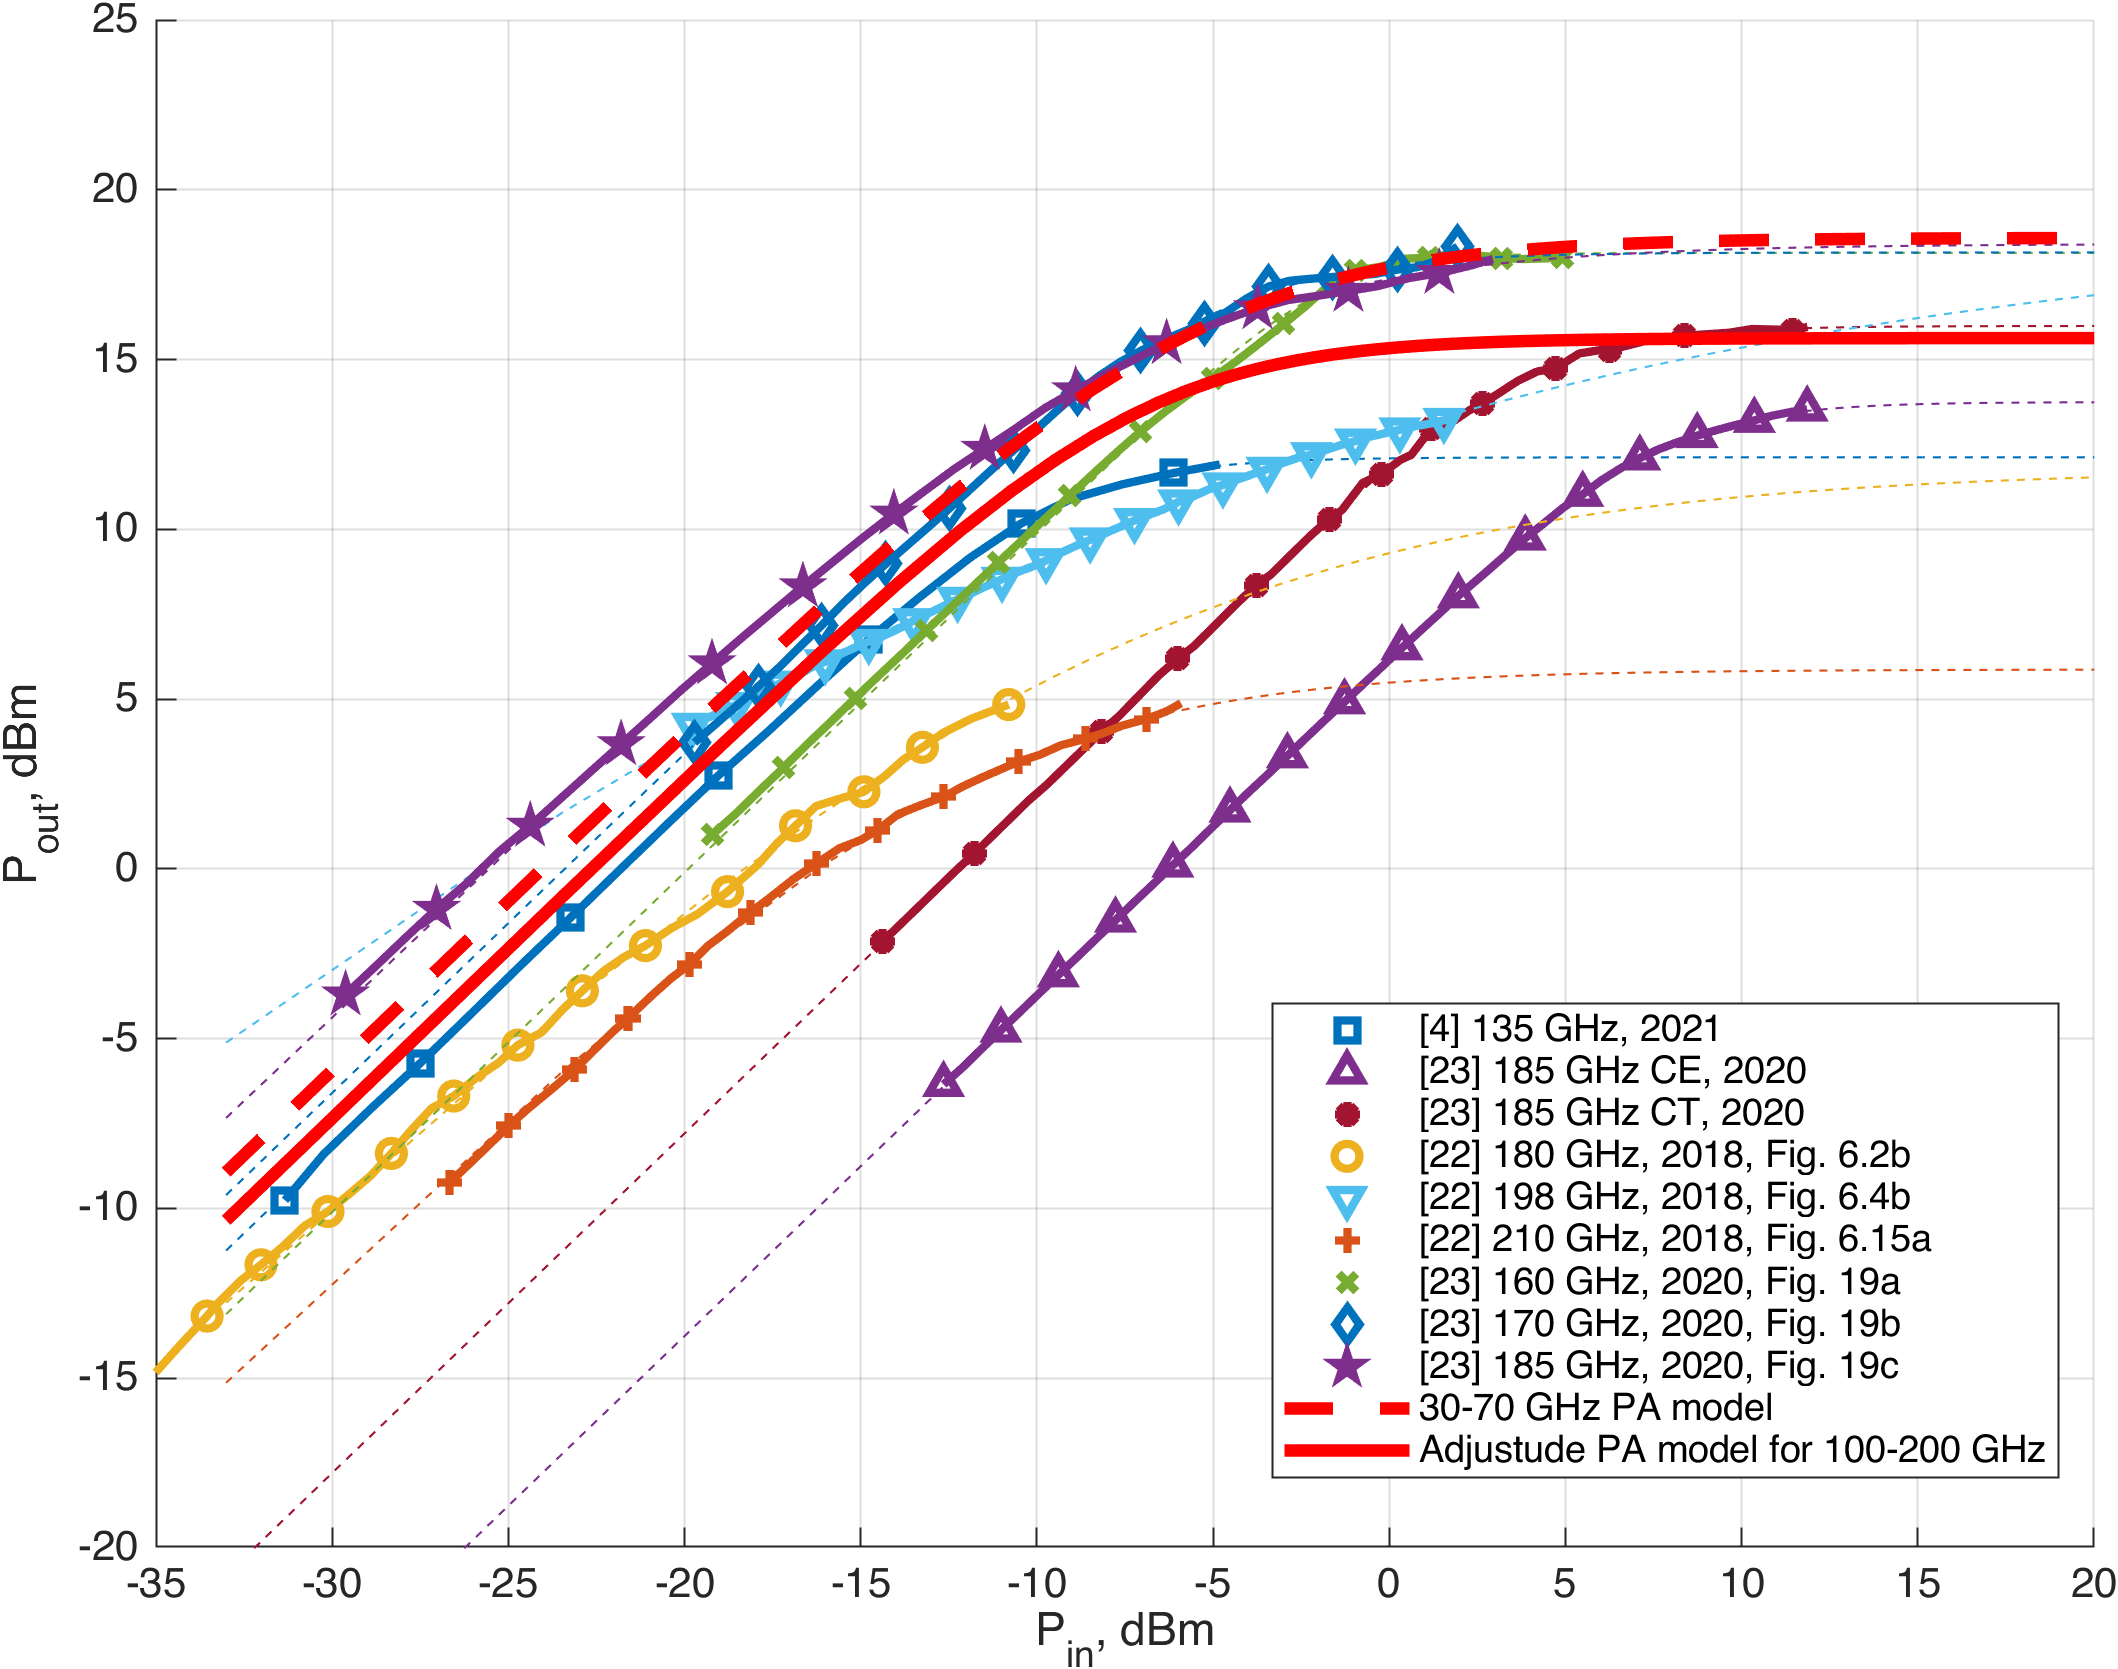
\includegraphics[width=0.95\linewidth]{figs/pacomparison.png}
    \caption{АХ усилителей на основе данных из
    \cite{zhang2021}\cite{amadorey2018}\cite{aliyun2020}, а также
    модель 30-70 ГГц \cite{nokia163314} и полученная усредненная модель
    для диапазона 100-200 ГГц}
    \label{fig:pa_research_mean}
\end{figure}

Извлеченные кривые амплитудных характеристик были аппроксимированы при
помощи модели Раппа \ref{eq:Rapp} (см. рис. \ref{fig:pa_research_mean} -
пунктирные линии), что позволило собрать параметры УМ для дальнейшей
обработки. Полученные значения параметров модели, а также частота и
технология для рассматриваемых усилителей приведены в Таблице
\ref{tab:pa_params}. 

\begin{table}[h]
    \centering
    \begin{tabular}{llcccc}
        \hline
    Источник              & Технология   & Частота, ГГц & $G$  & $V_{sat}$ & $p$ \\ \hline
    \cite{zhang2021}      & 28-нм CMOS   &  135         & 12.26 & 0.9      & 1.93  \\
    \cite{amadorey2018} Рис. 6.2b  & 35-нм mHEMT      &  180  & 10.84 & 0.87 & 0.52 \\
    \cite{amadorey2018} Рис. 6.4b  & 50-нм mHEMT      &  198  & 41.19 & 1.99 & 0.26  \\
    \cite{amadorey2018} Рис. 6.15a & 35-нм GaAs mHEMT &  210  & 7.89  & 0.44 & 0.9  \\
    \cite{aliyun2020} CT       &  130-нм SiGe BiCMOS CT        & 185 & 2.05  & 1.09 & 2.03  \\
    \cite{aliyun2020} CE       & 130-нм SiGe BiCMOS CE         & 185 & 4.08  & 1.41 & 1.91  \\
    \cite{aliyun2020} Рис. 19a & 130-нм SiGe BiCMOS 3-stage CT & 160 & 9.88  & 1.81 & 2.75  \\
    \cite{aliyun2020} Рис. 19b & 130-нм SiGe BiCMOS 3-stage CT & 170 & 14.8  & 1.81 & 1.56  \\
    \cite{aliyun2020} Рис. 19c & 130-нм SiGe BiCMOS 3-stage CT & 185 & 19.29 & 1.86 & 0.87  \\\hline
    \end{tabular}
    \caption{Параметры модели Раппа для УМ в диапазоне частот 100-200 ГГц
    на основе экспериментальных данных и исследований}
    \label{tab:pa_params}
\end{table}

\subsubsection{Параметры новой модели для диапазона частот 100-200 ГГц}
Для исследования применимости нового метода компенсации в диапазоне 100-200
ГГц необходима соответствующая модель УМ, для начальной имплементации ее в
систему с целью внесения соответствующих искажений в сигнал, и последующей
компенсацией внесенных искажений на приемнике. 

Имеющаяся модель \cite{nokia163314} подходит только для диапазона  30-70
ГГц, в нашем случае интерес представляет работа при более высоких частотах.
Модель для 100-200 ГГц была создана путем усреднения параметров $G,
V_{sat}, p$ рассмотренных УМ в соответствующем диапазоне частот (см. Таблицу
\ref{tab:pa_params}). Полученные усредненный параметры для модели Раппа
приведены в \ref{eq:rapp_p100200}.
\begin{equation}
    G = 13.59, \quad V_{sat} = 1.35, \quad p = 1.41
    \label{eq:rapp_p100200}
\end{equation}
Усредненная характеристика была получена только для амплитудного искажения $F_{AM/AM}$,
модель фазовых искажений была выбрана аналогичной модели для 30-70 ГГц.

